\documentclass[11pt,a4paper]{ivoa}
\input tthdefs

\usepackage{array}
\usepackage{tabulary}  % for nicer tables
\usepackage{calc}
\usepackage{placeins}
\setlength\extrarowheight{2pt}

\newcolumntype{L}{>{\centering\arraybackslash}m{3cm}}

\title{Model Instances in Votables}

% see ivoatexDoc for what group names to use here
\ivoagroup{DM}

\newcommand{\TODO}[1]{%
    \noindent%
    \colorbox{todocolor}{%
            \parbox{0.85\linewidth}{\sffamily \textbf{TODO:}\\
            #1}
    }%
    \vspace{2pt}
}

\newcommand{\note}[1]{%
    \noindent%
    \textcolor{darkgrey}{{\sffamily Note:} \emph{#1}}%
}

\newcommand{\comment}[1]{%
    \noindent%
    \textcolor{red}{{\sffamily Comment:} \emph{#1}}%
}

%%%%%%%%%%%%%%%%%%%%%%%%%%%%%%%%%%%%
% XML syntax coloration and formatting
%
\definecolor{todocolor}{rgb}{1,1,0.8}
\definecolor{darkred}{rgb}{0.6,0,0}
\definecolor{rose}{rgb}{1.0,0.88,0.88}
\definecolor{darkgrey}{rgb}{0.35,0.35,0.35}
\definecolor{gray}{rgb}{0.4,0.4,0.4}
\definecolor{darkblue}{rgb}{0.0,0.0,0.6}
\definecolor{maroon}{rgb}{0.5,0,0}
\definecolor{cyan}{rgb}{0.0,0.6,0.6}
\definecolor{darkgreen}{rgb}{0,0.5,0}
\definecolor{lightblue}{rgb}{0.0,0.0,0.9}
\definecolor{mauve}{rgb}{0.58,0,0.82}
 \lstloadlanguages{XML}
 \lstdefinestyle{XML}{
    captionpos=b,
    basicstyle=\tiny
}

 \lstset{flexiblecolumns=true,
            columns=fullflexible,
            tagstyle=\ttfamily,
            showstringspaces=False,
            basicstyle=\tiny, 
            captionpos=b,
            frame=single,
            commentstyle=\color{gray}\upshape}
\lstdefinelanguage{XML}
{
  morestring=[s][\color{mauve}]{"}{"},
  morestring=[s][\color{black}]{>}{<},
  morecomment=[s][\color{gray}]{!--}{-->} ,
  stringstyle=\color{black},
  identifierstyle=\color{lightblue},
  keywordstyle=\color{darkgreen},
  morekeywords={xmlns,xsi,status,name,url, ref,tableref,dmid,dmref,dmrole,dmtype,value }% list your attributes here
   }


%%%%%%%%%%%%%%%%%%%%%%%%%%%
% Document core
%
\author{François Bonnarel}
\author{Gilles Landais}
\author{Laurent Michel}
\author{Jesus Salgado}
\author{Gerard Lemson}

\editor{Laurent Michel}
\editor{Mark Cresitello-Dittmar}


% \previousversion[????URL????]{????Concise Document Label????}
\previousversion{This is the first public release}
       

\begin{document}

\begin{abstract}
Model Instances in VOTables (MIVOT) defines a syntax to map VOTable data to any model serizalized in VODML.
The annotation operates as a bridge between the data and the model.
It associates the column/param metadata from the VOTable to the 
data model elements (class, attributes, types, etc.) of a standardized IVOA data model, expressed in the Virtual Observatory Data Modeling Language (here after VO-DML).
It also brings up VOTable data or metadata that were possibly missing in the table metadata.

The data model elements are grouped in an independent annotation block complying with the MIVOT XML syntax.
This annotation block is added as an extra resource element at the top of the VOTable result resource. 
The MIVOT syntax allows to describe a data structure as a hierarchy of classes. It is also able to represent relations and composition between them.It can also build up data model objects by aggregating instances from different tables of the VOTable.

Missing metadata can also be provided using MIVOT, for instance by completing coordinate system description, or by providing curation tracing.

The annotation block is made of re-usable bricks that facilitate the developement of tools on both client and server sides.
The adopted design does not alter the original VOTable content. 
The backward compatibility is preserved thanks to the limited impact of the annotations on legacy clients.
\end{abstract}


\section*{Acknowledgments}
We would like to thank all the people who have contributed to this standard, starting with the authors of the VO Data Modeling Language who have introduced the concepts developed here.
We would also like to thank all contributors of the "Source Data Model" session held at the Paris Interop Meeting in 2019, as well as all members of the IVOA Time Domain Interest Group and the participants to the Data Model workshop we ran in Spring 2021. All helped us to refine our use-cases.
Finally, we say a big thank you to the CDS members who spent time for assessing how such an annotation procedure could improve their VO services.
This acknowledgement does not mention individuals, as the list would be too long, especially the many interns who contributed to this project.

\section*{Conformance-related definitions}

The words ``MUST'', ``SHALL'', ``SHOULD'', ``MAY'', ``RECOMMENDED'', and
``OPTIONAL'' (in upper or lower case) used in this document are to be
interpreted as described in IETF standard RFC2119 \citep{std:RFC2119}.

The \emph{Virtual Observatory (VO)} is a
general term for a collection of federated resources that can be used
to conduct astronomical research, education, and outreach.
The \href{http://www.ivoa.net}{International
Virtual Observatory Alliance (IVOA)} is a global
collaboration of separately funded projects to develop standards and
infrastructure that enable VO applications.

\pagebreak
\section{Introduction}


The first purpose of a model is to provide, for a particular domain, a formal description of the quantities relevant to that domain and how they relate to each other.
The second purpose is to facilitate the interoperability between  different stakeholders involved in the domain. The interoperability consists in arranging exchanged data 
so that any client can understand it without being concerned with its origin thus allowing the same code to process and compare data coming from different archives.  
In other words, the more faithful is the data representation towards the data model, the better is the interoperability.
The challenge for the VO ecosystem is to design the best way to map various data on standard models while respecting the existing frameworks, protocols and data formats.

We could imagine to develop a new data container specific for that purpose but any solution that ignores the existing assets would be utterly useless and would have no chance of being accepted.
The model mapping solution must be based on VOTables since VOTable  \citep{2019ivoa.spec.1021O} is the standard data container within the VO.
Unfortunately, if the VOTable schema allows a very good description of tabular data, it is not well suited for rendering views of complex data models.
In the case of simple DAL protocols, this limitation has been worked around by specifying the metadata that must be present in the query responses; the model mapping is thereby defined by the standard.
This approach is no longer applicable for complex models such as Cube or Provenance data models for which the data tree may vary from one instance to another.

The basis on which the standard is designed is threefold 1) the data content is apriori unknown (e.g. TAP response), 2) it has to be mapped on models that are not defined yet and 3) the data model metadata used for these serialized data must be fully contained within a VOTable context.
%It must also allow to bind native data with a model in a way that model-aware software can see it as model instances while maintaining the possibility to access them in their original layout.
The  standard should allow a model-aware software to create instances of objects described by the model by binding together native column data , and also warrant the direct access to table columns as planned in the original data serialization.


The VOTable schema supports an XML attribute for this purpose, a UType, that partially meets this function. 
UTypes are path-like strings (\texttt{m:a.b.c}) identifying model leaves. As there is no common rule to build UTypes,  each data model (e.g. Characterization, Obscore)  must come with its specific lists of UTypes. 

When used as \texttt{FIELD} attributes, UTypes allow one to connect particular columns to model leaves. This mapping method fits very well with the VOTable schema since it does not require any specific XML elements. It has however a number of limitations that have been discussed many times:

\begin{itemize}
  \item UTypes are labels attached to  a \texttt{FIELD} or \texttt{PARAM} that tells its role in the 
  model structure, typically a non cyclic graph. 
   \item There is no possibility for one  \texttt{FIELD} or \texttt{PARAM} to play multiple roles.
  \item UTypes are not intended to be parsed, so they only identify which role corresponds to a \texttt{FIELD}/\texttt{PARAM} , the 'leaf'  element in the data model hierarchy.
  It belongs to a restricted context : a class, a set of classes, a link to another class.
  % ??? mireille: some rephrasing needed here 
  %\item UTypes are not reusable, the same element used in different contexts or models have different UTypes; which hinders interoperability
  \item UTypes constrain to single-table serializations. All model elements must 
  be contained within the same VOTable TABLE.
  % mir ??? not clear enough : prov dm has many tables with well defined utypes 
 
  \item UTypes do not support annotating the VOTable content towards multiple models 
  (as TimeSeries or Catalog/Source for instance )
  % the utype is data model dependent , ok, by construction but the annotation also , no? 
  % not sure it is this an important point to mention here ?
\end{itemize}

The UType approach could have been extended to overcome these drawbacks, but it has been decided to move forward a solution closer to the \texttt{VODML} \citep{2018ivoa.spec.0910L} concepts. 
% mireille : A more general approach to provide a global data model description from the data model UML diagram was adopted.
 \texttt{VODML} is a meta-model that gives a standard way to express VO models and to provide a machine-readable description in an XML document.
In \texttt{VODML},  model leaves are no longer identified by simple strings like UTypes do, but by the role they play in a given location in the model hierarchy.
As a consequence, any annotation mechanism based on \texttt{VODML} and preserving the model hierarchy will be able  to provide a data representation faithful to that model.
% this conclusion seems too quick to me here

The basis of MIVOT is to insert into the VOTable, an XML block complying with the 
model structure and containing references to the actual data.
These blocks are designed in such a way that a model-aware client can build  model instances by copying that structure and by resolving the references. 
Other clients can just ignore them and rely on the FIELD/PARAM and GROUP structures provided with VOTable format. 

%MOVED from section2

%The meta-data currently supported by the  VOTable standard gives a very good description of the table field content. 
%There is however not suitable way to specify the exact role played by a given quantity in a particular context yet.

%There is also no way to describe how different quantities or different data tables relate to each other either.
%UTypes have been proposed to fill these gaps, but the difficulty to define a standard method to build them in the general case of non-hierachical models caused this approach not to be used.
%Actually, both role specifications and quantity associations are parts of the modelling effort and our need is a bridge between model leaves and data columns that allows users to get a model view on data tables. (%NFB Hummm. Is that only for leaves ? Or also for higher levels ?)
%This is essential to get a good  understanding of complex data.




\subsection{Role within the VO Architecture}

\begin{figure}[h]
\centering

% As of ivoatex 1.2, the architecture diagram is generated by ivoatex in
% SVG; copy ivoatex/archdiag-full.xml to archdiag.xml and throw out
% all lines not relevant to your standard.
% Notes don't generally need this.  If you don't copy archdiag.xml,
% you must remove archdiag.svg from FIGURES in the Makefile.

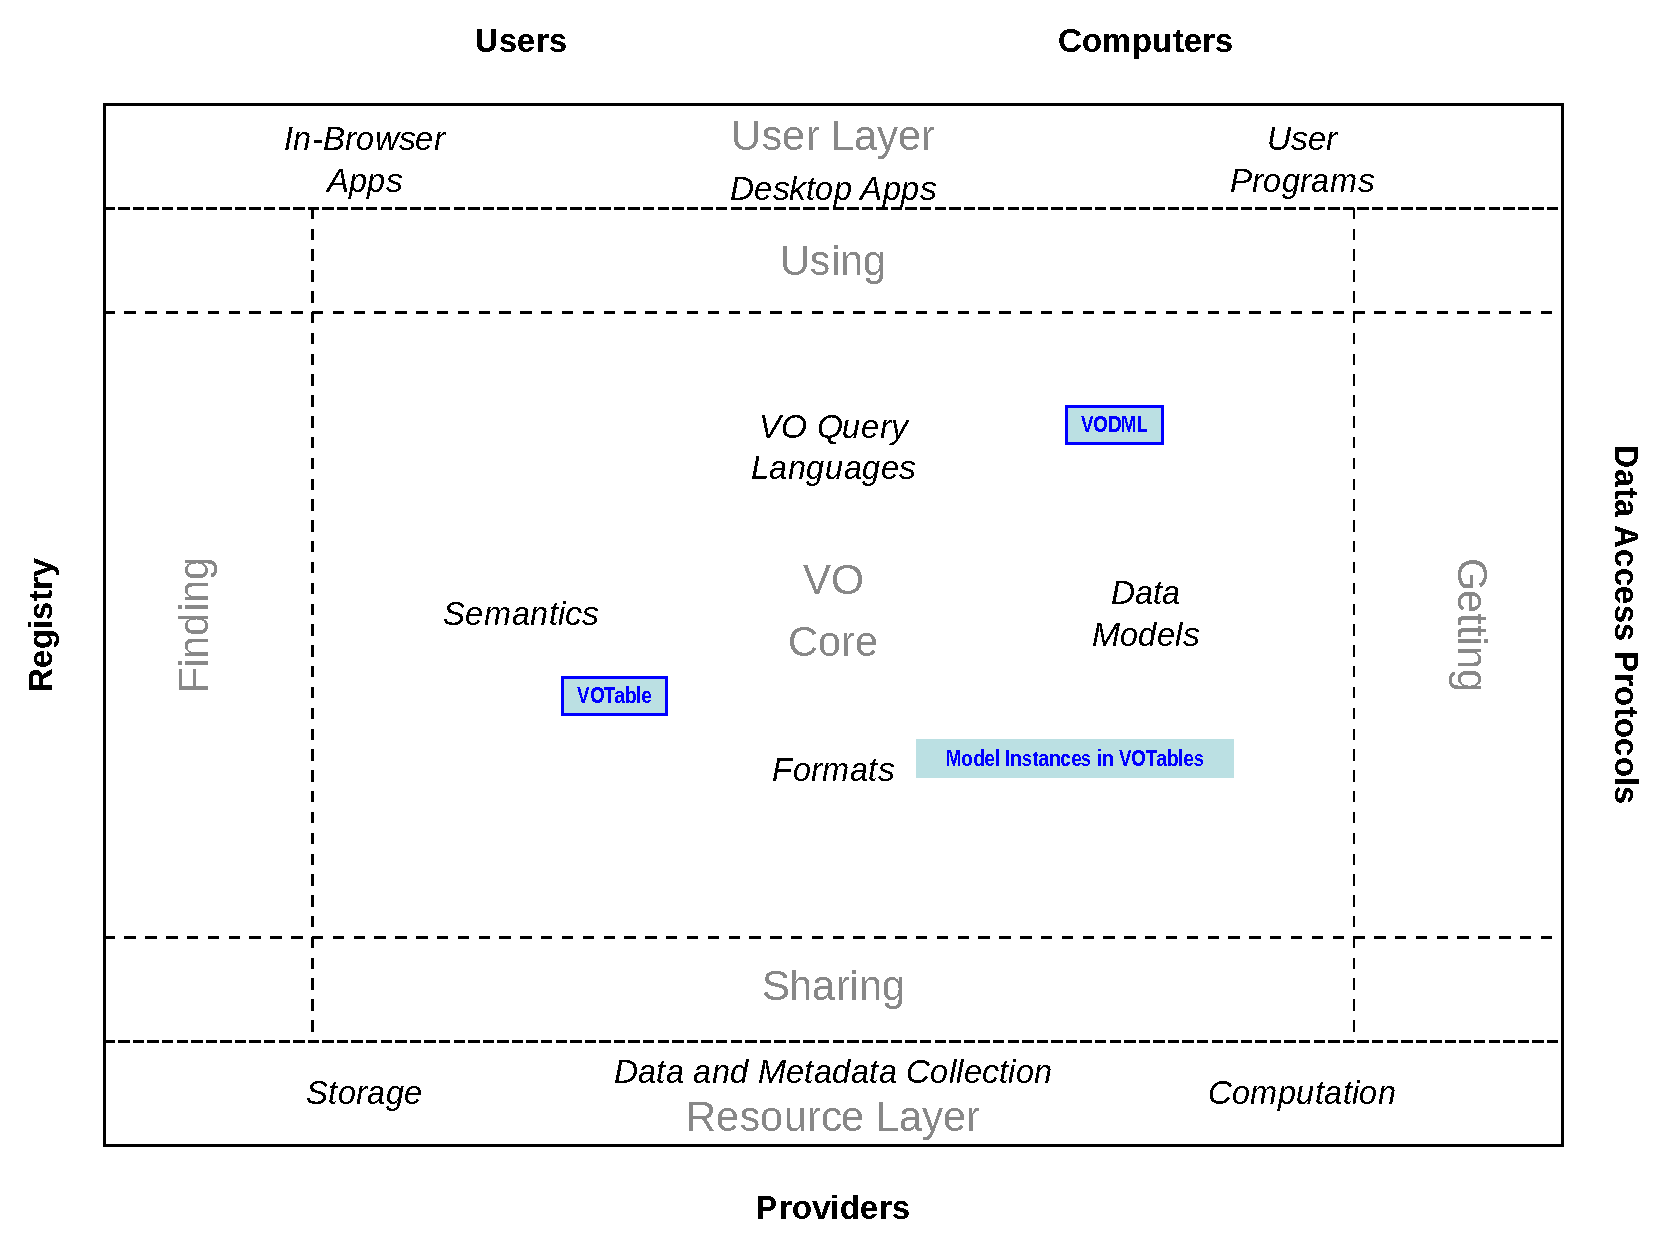
\includegraphics[width=0.9\textwidth]{role_diagram.pdf}
\caption{Architecture diagram for this document}
\label{fig:archdiag}
\end{figure}

Fig.~\ref{fig:archdiag} shows the role this document plays within
the IVOA architecture \citep{2010ivoa.rept.1123A}.


\pagebreak
\section{Use Cases and Requirements}

\subsection{Use Cases}
The aim of the mapping syntax is to enable services to associate a model view to searched data.
Model views can be applied either to legacy data or 
The usage of such model views can range for a simple enhancement of the meta-data up to representation of full model instances.
\begin{itemize}
  \item 
\end{itemize} 


Mapping legacy on a model

data enhance column description

Give the role of column groups

Allows the map complex data structures on legacy data


A step toward a better DM integration in the VO consists in enabling services to annotate
legacy data by providing complete model
views. This requires the server to operate a post-processing inserting into VOTables
annotations that bind data columns with model leaves. .

The mapping syntax allows to map data on any model compliant with VODML. 
These annotations are built as leading XML blocks in VOTables. 
Annotation blocks denote the model structure and contain references to the appropriate table
FIELDs. Model-aware clients can build model instances just by reading the annotation
block and by resolving the FIELD references to get the model leaf values. 

The server must be able to automatically generate such annotations. For this, it
must check that the selected columns match with the model definitions and thus can be
mapped on that model. To operate the mapping, the server needs further information
such as coordinate frames and data profile resources giving the binding between table
columns and model leaves. A prototype (Louys et al. 2021) implementing this feature
has been demonstrated 3.

Allow VOTable to carry complete model instances

TAP services can also be used to host model instances. In this case, we must not
map data on a model anymore but we have to do a real object relational mapping.
However, proposing a common ORM schema is not on the VO roadmap. The work
around strategy is to propose one specific standard per model. This has been done first
for ObsTAP (Tody et al. 2011) which flattens the ObsCore model on one table. This is
also the case for ProvTAP 4 which proposes a relational view for Provenance (Servillat
et al. 2020) data. A prototype (ProvHiPS) tracing the provenance of HST HiPS tiles
has been implemented demonstrated. As the model mapping is defined by a standard,
there is no need to add extra information to the TAP service. Both TAP\_SCHEMA
content and meta-data defined in that standard provide all pieces of information needed
to construct model instances from query results. There are however 2 major issues: 1)
Provenance instances cannot be serialized in one single table; in order to solve this issue
resulting VOTable documents must either contain multiple tables or provide a flattened
view of the model itself (namely last step provenance) 2) The client must be able to tell
the server it is searching Provenance instances.



\subsection{Requirements}
\begin {itemize}
  \item Shy annotation % mir :is this term clear enough in the VO
  
  	Model annotations enter into a workflow which has been working very well for years. As a matter of fact, the first requirement is to keep 
	%any existing stakeholder unbroken.  % mir stakeholders are the big projects : XMM, CDS, HEASARC, ESO , etc ...
	legacy services operational and not to require a full rebuilt of existing archives. Therefore: 
	
  \begin {itemize}
    \item Annotation must not alter the VOTable content.
    \item Annotation blocks must be located in a way that it can easily be skipped by model-unaware clients.
    \item The vocabulary in the annotation name-space must not overlap with the VOTable elements (names or attributes)    
    \item The annotation syntax must be able to inform the client about the status of the annotation process.
  \end {itemize}
  
  \item Schema and validation:
  \begin {itemize}
     \item The content of the annotation block must be validated according to a specific schema.
    \item The annotation schema must be independent from the VOTable schema.
    \item The evolution of the annotation schema must not impact the VOTable schema.
    \item The evolution of the VOTable schema must not impact the annotation schema.
    \item The annotation syntax must be validated using the usual tools, i.e. without using specific compilers.
    \item Validators are not meant to check whether references can be resolved. Clients are in charge of handling possible inconsistencies.
  \end {itemize}
  
  \item Model agnostic behavior:
  \begin {itemize}
    \item The annotation syntax must be able to map data on any \texttt{VODML} compliant model
    \item The annotation syntax must allow clients to use their own strategy to consume mapped data, so they could:
      \begin {itemize}
        \item just ignore it
        \item pick some elements of interest 
        \item pick model metadata and process the sequence of data rows as usual
        \item pick whole model instances     
        %mir whole ??  instances of the whole model ? 
        %mir does this means the current votable instanciates all the classes of the model ? very seldom i guess
        %mir  or select all serialized instances that are tagged with data model metadata in order to instanciate corresponding data model objects 
      \end {itemize}
  \end {itemize}
  
  \item On the fly annotation status:
      \begin {itemize} 
          \item Clients connecting TAP services registered as delivering annotated data must get VOTable with annotation blocks in any case. 
          \item Clients must be informed on the execution status of the annotation process.     
          \item Clients must be informed of the data model name and version used for the annotation  
       \end {itemize}

\end {itemize}



% use XML formatting for listings
\lstset{language=XML}

\pagebreak
\section{Relation to VOTable}

The data model annotation will reside within the scope of a VOTABLE V1.1+.


\noindent \textbf{Location}

The mapping block:
\begin{itemize}
\item MUST be contained in a VOTable RESOURCE with \texttt{type="meta"}. This extra feature is consistent with VOTable xml schema RESOURCE type definition and doesn't require any modification in the xml schema.
\item which MUST be the first child of a RESOURCE with \texttt{type="results"}.
\item there MUST be no more than one mapping block per 'results' RESOURCE.
\end{itemize}

The scope of the mapping block is the whole content of the 'results' RESOURCE. \newline

\noindent \textbf{Namespace}

The mapping element must be isolated from the VOTable elements by a name space set as an attribute of the \texttt{VODML} element.

\begin{lstlisting}[caption={Mapping block in a VOTable},language=XML]
<VOTABLE xmlns="http://www.ivoa.net/xml/VOTable/v1.3" 
         xmlns:xsi="http://www.w3.org/2001/XMLSchema-instance" version="1.3">
  <RESOURCE type="results">
    <RESOURCE type="meta">
      <VODML xmlns="http://www.ivoa.net/xml/merged-syntax">
        ...
      </VODML>
    </RESOURCE>
    <TABLE name="myDataTable">
      ....
    </TABLE>
  </RESOURCE>
</VOTABLE>
\end{lstlisting}


\pagebreak
\section{Syntax}

\subsection{Overview}

The syntax has been designed %to use as few XML elements as possible and to rely on XML attributes to setup the element behavior in a particular context.
as a restricted but still complete set of XML elements. It relies on XML attributes to setup the element behavior in a particular context.
As shown in table \ref{tbl:syntax-ele} the mapping elements  are used %can be grouped 
in three different scopes. There are only three elements for the models structure itself. We assume that any data hierarchy  can be represented by a combination of collections  \texttt{COLLECTION}, tuples  \texttt{INSTANCE}, and simple values  \texttt{ATTRIBUTE}. The others elements are either to set the mapping block structure or to connect data to each other.

\begin{table}[!htbp]
\small
\centering
\begin{tabulary}{\linewidth}{|c|J|}       
       \hline 
            \textbf{Scope} & 
            \textbf {Elements}\\
       \hline         
       \hline  
             Data modeling tags & 
             \texttt{ATTRIBUTE} \texttt{INSTANCE} \texttt{COLLECTION} \\
       \hline  
             Mapping block structure & 
             \texttt{VODML} \texttt{MODEL} \texttt{REPORT} \texttt{TEMPLATES} \texttt{GLOBALS} \\
       \hline  
             Data references and identification & 
             \texttt{REFERENCE} \texttt{JOIN}  \texttt{FOREIGN\_KEY} \texttt{PRIMARY\_KEY} \texttt{WHERE} \\
       \hline
     \end{tabulary}
     \caption{Mapping elements grouped by scopes.} 
     \label{tbl:syntax-ele}
\end{table}


As shown in Table \ref{tbl:syntax-att} and following the \texttt{VODML} pattern, any model node is characterized by a role  \texttt{@dmrole}  and a type  \texttt{@dmtype}.  All of the other attributes are used to bind data with either VOTable elements or other mapping elements.
 
\begin{table}[!htbp]
\small
\centering
\begin{tabulary}{\linewidth}{|c|J|}       
       \hline 
            \textbf{Scope} & 
            \textbf {Attributes}\\
       \hline         
       \hline  
             Model related & 
             \texttt{@name} \texttt{@uri} \\
       \hline  
             Modeled node related & 
             \texttt{@dmrole} \texttt{@dmtype} \\
       \hline  
             Related to attribute values & 
             \texttt{@value} \texttt{@unit} \texttt{@arrayindex} \\
       \hline  
             Related to VOTable elements & 
             \texttt{@tableref} \texttt{@ref} \\
       \hline  
             Mapping element identification& 
             \texttt{@dmref} \texttt{@dmid} \texttt{@url} \texttt{@sourceref} \texttt{@primarykey} \texttt{@foreignkey} \\
       \hline
     \end{tabulary}
     \caption{Attributes of mapping elements grouped by scopes.} 
     \label{tbl:syntax-att}
 \end{table}
 
 


  \begin{figure}[h]
    \begin{center}
      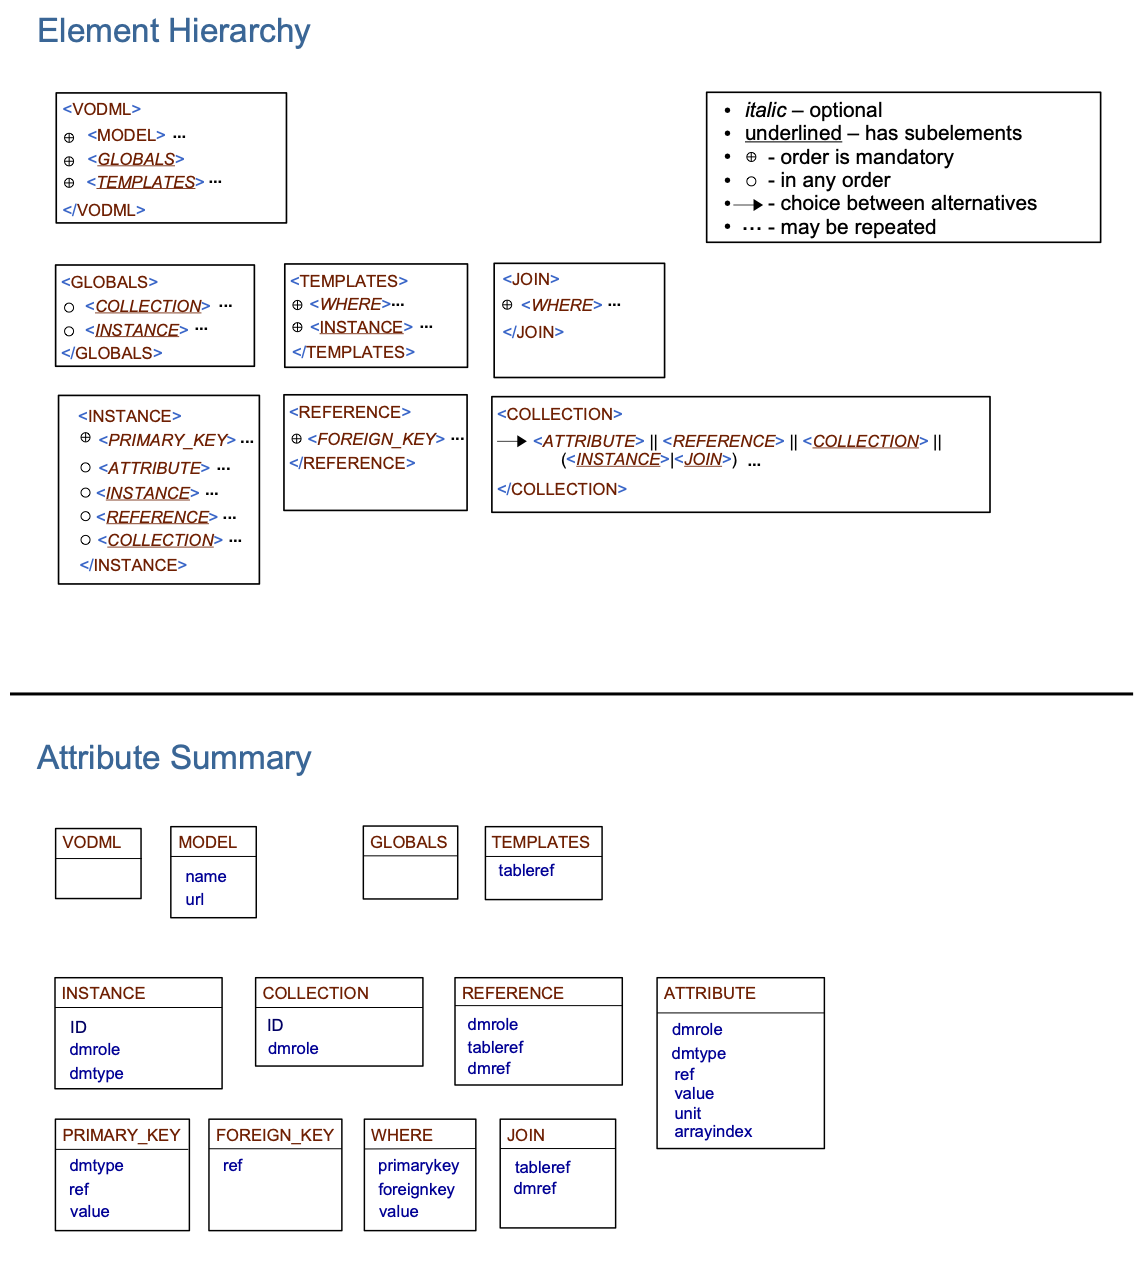
\includegraphics[width=1.2\textwidth]{mivot-summary.png}
      \caption{Annotation Syntax Summary.}
      \label{fig:summary}
    \end{center}
  \end{figure}


\subsection{Reader's Guide}

In the following normative subsections, all mapping patterns are illustrated with XML snippets.
Most of these excerpts are taken out of a complete VOTable listed in appendix \ref{appendix_A}.
The others are out of the box, they refer to model elements or VOTable metadata that do not exist 
but that have been chosen to achieve better readability. 
Readers can have a look at \url{https://github.com/ivoa-std/ModelInstanceInVot/tree/master/data-sample} 
to inspect most of them in a context of real data.



\pagebreak
\subsection{VODML}
The \texttt{VODML} element is the top level container for the mapping elements for a single VOTable RESOURCE.
When the mapping \texttt{@status} attribute of the \texttt{REPORT} is set to KO, the other children mapping elements are optional.

\begin{lstlisting}[caption={Example \texttt{VODML} mapping block.},language=XML]
<VODML xmlns="http://www.ivoa.net/xml/mivot">
  <REPORT status="OK"/>
  <MODEL>  ...  </MODEL>
  <GLOBALS>  ...  </GLOBALS>
  <TEMPLATES>  ...  </TEMPLATES>
   ...
</VODML>
\end{lstlisting}

\begin{table}[!htbp]
  \small
  \centering
  \begin{tabulary}{\linewidth}{|c |c |c|}
    \hline 
        \textbf{Element} &
        \textbf{Position} &
        \textbf{Occurs}\\
    \hline
    \hline  
      \texttt{REPORT} &           
      1 &           
      0-1\\
    \hline  
      \texttt{MODEL} &           
      2 &           
      0-*\\
    \hline    
      \texttt{GLOBALS} &           
      3 &           
      0-*\\
    \hline  
      \texttt{TEMPLATES} &           
      4 &           
      0-*\\
    \hline 
  \end{tabulary}
    \caption{Allowed children for \texttt{VODML}.} 
    \label{tbl:vodml-children}
\end{table}



\FloatBarrier

\subsection{REPORT}
Services providing annotated responses must use the \texttt{REPORT}  element to tell the client whether the annotation process succeeded or not.

\begin{itemize}
\item \texttt{REPORT} is not mandatory.
\item It must be the first \texttt{VODML} child if present.
\end{itemize}



\begin{lstlisting}[caption={\texttt{REPORT} example for an annotation failure},language=XML]
<VODML	xmlns="http://www.ivoa.net/xml/merged-syntax">
	
	<REPORT status="KO">
	    The annotation process failed
	</REPORT>
	<!-- 
	   No other annotation
	  -->	
</VODML>
\end{lstlisting}

\begin{lstlisting}[caption={\texttt{REPORT} example for an valid annotation},language=XML]
<VODML	xmlns="http://www.ivoa.net/xml/merged-syntax">
	
	<REPORT status="OK">
	    The annotation process succeed
	</REPORT>

	<MODEL name="model" url="http://aaaaaa" />
	<MODEL name="model" />
	
	<GLOBALS>...</GLOBALS>
	<TEMPLATES ...>
	   ...
	 </TEMPLATES>
	
</VODML>
\end{lstlisting}


\begin{table}[!htbp]
  \small
  \centering
  \begin{tabulary}{\linewidth}{|c|J|}       
    \hline 
         \textbf{Attribute} & 
         \textbf {Role}\\
    \hline
    \hline  
         @status  & 
        Status of the annotation process; must be either \texttt{OK} or \texttt{KO} \\
    \hline 
  \end{tabulary}
  \caption{\texttt{REPORT} attributes} 
  \label{tbl:report-att}
\end{table}


\FloatBarrier
 
\subsection{MODEL}
A VOTable can provide serializations for an arbitrary number of data model
types. In order to declare which models are represented in the file, data
providers must declare them through the \texttt{MODEL} elements.
Only models that are used in the file must be declared. A model is
used if at least one element in the mapping block refer to it. In other terms, only models that define vodml-ids used in the
annotation must be declared.

\begin{lstlisting}[frame=single,caption={Example \texttt{MODEL} mapping block},style=XML,basicstyle=\tiny]
<dm-mapping:VODML>
  <dm-mapping:MODEL name="sample-ext"
                     url="https://www.myorg.net/models/SampleExt-v1.0.vo-dml.xml" />
  <dm-mapping:MODEL name="sample" url="https://www.ivoa.net/xml/DNE/Sample-v1.0.vo-dml.xml" />
  <dm-mapping:MODEL name="ivoa"   url="https://www.ivoa.net/xml \texttt{VODML} IVOA-v1.vo-dml.xml" />
</dm-mapping:VODML>
\end{lstlisting}

\begin{table}[!htbp]
  \small
  \centering
  \begin{tabulary}{\linewidth}{|c|J|}       
    \hline 
         \textbf{Attribute} & 
         \textbf {Role}\\
    \hline
    \hline  
         \texttt{@name}  & 
         Name of the mapped model as declared in the \texttt{VODML} XML model serialization.  This attribute MUST not be empty and forms the prefix used in dmrole/dmtype tags of elements from that model.  \\
    \hline 
         \texttt{@url} & 
         URL to the vo-dml serialization of the model. If present, this attribute MUST not be empty.\\
    \hline 
  \end{tabulary}
  \caption{\texttt{MODEL} attributes} 
  \label{tbl:model-att}
\end{table}


\begin{table}[!htbp]
  \small
  \centering
  \begin{tabulary}{\linewidth}{|c |c |J|}
    \hline 
        \textbf{@name} &
        \textbf{@url} &
        \textbf{Pattern}\\
    \hline      \hline  
        MAND &           
        OPT &           
        Unique attribute pattern supported by \texttt{MODEL}\\
    \hline 
  \end{tabulary}
  \caption{Valid attribute patterns for  \texttt{MODEL}} 
  \label{tbl:model-pattern}
\end{table}

\FloatBarrier

\subsection{GLOBALS}
The \texttt{GLOBALS} block holds model instances or collections of model instances 
that are not connected with any table column. 

The instances or collections contained in \texttt{GLOBALS} have a global scope. They can be
referenced by other instances anywhere in the mapping block.  
They must only contain literal values.
They must not refer to VOTable \texttt{FIELDS} or \texttt{PARAM} either.  \\ 

Related instances may be grouped within \texttt{COLLECTION} blocks to enable selection
via the MIVOT \texttt{JOIN} mechanism.  
See \texttt{COLLECTION} subsection for more details.

\begin{lstlisting}[caption={Example \texttt{GLOBALS} block (see line~\ref{GLOBALS_snippet} in Appendix~\ref{appendix_A} ) which contains a collection of coordinate systems.},language=XML]
<VODML xmlns:dm-mapping="http://www.ivoa.net/xml/mivot" >
    <REPORT status="OK">Mapping compiled by hand</REPORT>
    <MODEL... />
    <!--	             
        place holder for singular data model instances not associated with a singular VOTabme TABLE
     -->
    <GLOBALS>
        <!--
          Container for the coordinate systems
         -->
        <COLLECTION dmid="IDCoordinateSystems" dmrole="" >
           ...
        </COLLECTION>
        ...
    </GLOBALS>
    ...
 </VODML>
\end{lstlisting}


\begin{table}[!htbp]
  \small
  \centering
  \begin{tabulary}{\linewidth}{|c |c |c|}
    \hline 
        \textbf{Element} &
        \textbf{Position} &
        \textbf{Occurs}\\
    \hline
    \hline
        \texttt{INSTANCE} &
        Any &
        0-*\\
    \hline
        \texttt{COLLECTION} &
        Any &
        0-*\\
    \hline
  \end{tabulary}
  \caption{Allowed children elements for \texttt{GLOBALS}.} 
  \label{tbl:globals-children}
 \end{table}

\FloatBarrier

\subsection{TEMPLATES}
The \texttt{TEMPLATES} block defines a template for deriving multiple data model instances,
one for each row of the associated VOTable \texttt{TABLE}.  A subset of the associated
\texttt{TABLE} rows may be selected using the \texttt{WHERE} syntax element.

\begin{lstlisting}[caption={Example of a \texttt{TEMPLATES} block mapping the rows of the table \texttt{Results} (see line~\ref{TEMPLATES_snippet} in Appendix~\ref{appendix_A}).
Each row of the table named \texttt{Results} is be mapped on an instance of the VO-DML type \texttt{cube:NDPoint}.
Instances mapping a table row do not play any particular role.},language=XML]
<VODML xmlns="http://www.ivoa.net/xml/mivot">
    ...
    <GLOBALS>
    ...
    </GLOBALS>
    <!--
       Mapping of the rows of the table Results
     -->  
    <TEMPLATES tableref="Results">
        <INSTANCE dmid="IDtsIDdata" dmrole="" dmtype="cube:NDPoint">
            <COLLECTION dmrole="cube:NDPoint.observable">
                <INSTANCE dmtype="cube:Observable">
                    <ATTRIBUTE dmrole="cube:DataAxis.dependent" dmtype="ivoa:boolean" value="False"/>
                    ...
                </INSTANCE>
            </COLLECTION>
            ...
        </INSTANCE>
    </TEMPLATES>
</VODML>
\end{lstlisting}

\begin{table}[!htbp]
  \small
  \centering
  \begin{tabulary}{\linewidth}{|c|J|}
    \hline 
         \textbf{Attribute} & 
         \textbf {Role}\\
    \hline
    \hline  
         \texttt{@tableref} & 
         ID or name of the mapped VOTable \texttt{TABLE}. ID match takes precedence over name matches when resolving the reference. \\
    \hline 
  \end{tabulary}
  \caption{\texttt{TEMPLATES} attributes.} 
  \label{tbl:templates-att}
\end{table}

\begin{table}[!htbp]
  \small
  \centering
  \begin{tabulary}{\linewidth}{|c|J|}
    \hline 
        \textbf{@tableref} &
        \textbf{Pattern}\\
    \hline
    \hline  
        OPT &           
        If \texttt{@tableref} is not present, \texttt{TEMPLATES} maps the first \texttt{TABLE} of the \texttt{RESOURCE}\\
    \hline 
  \end{tabulary}
  \caption{Valid attribute patterns for  \texttt{TEMPLATES}.} 
  \label{tbl:templates-pattern}
 \end{table}

\begin{table}[!htbp]
  \small
  \centering
  \begin{tabulary}{\linewidth}{|c |c |c|J|}
    \hline 
        \textbf{Element} &
        \textbf{Position} &
        \textbf{Occurs} &
        \\
    \hline
    \hline  
        \texttt{WHERE}  &        
        1 &           
        0-* &
        The mapping applies to rows matching the \texttt{WHERE} condition only\\
    \hline    
        \texttt{INSTANCE} &           
        2 &           
        0-* &
        Mapped instance templates\\
    \hline 
  \end{tabulary}
  \caption{Allowed children for \texttt{TEMPLATES}.} 
  \label{tbl:templates-children}
\end{table}

\FloatBarrier

\subsection{COLLECTION}
    COLLECTION is a container element.  It is used in different contexts, each allowing a limited subset of elements for its content. 

    \begin{enumerate}
    \item{As child of INSTANCE}
      
      The COLLECTION serves as a container for elements with multiplicity $>$ 1.\\
      Examples of usage in this context would be:
      \begin{itemize}
        \item an array attribute
        \item a reference relation with multiplicity $>$ 1
        \item a composition relation with multiplicity $>$ 1
      \end{itemize}
      
    \item{As child of GLOBALS}
          
      The COLLECTION serves as a proxy for TABLE, grouping common INSTANCES for selection by PRIMARY/FOREIGN\_KEY.
      Examples of usage in this context would be:
      \begin{itemize}
        \item a set of photometry filters, which apply to various rows of a photometric data table, based on the value of the 'band' column.
        \item a set of Dataset metadata instances, which apply to various rows of a photometric data table, based on the value of the 'band' column.
      \end{itemize}
          
    \item{As child of COLLECTION}

          The use-case for this is unclear
        
    \end{enumerate}
   
\begin{lstlisting}[frame=single,caption={Example of COLLECTION child of INSTANCE},style=XML,basicstyle=\tiny]
<dm-mapping:INSTANCE dmtype="model:Thing">
    <dm-mapping:COLLECTION dmrole="model:Thing.elems">
        <dm-mapping:ATTRIBUTE dmtype="model:Foo" value="100" />
        <dm-mapping:ATTRIBUTE dmtype="model:Foo" value="110" />
    </dm-mapping:COLLECTION>
</dm-mapping:INSTANCE>
\end{lstlisting}   

\begin{lstlisting}[frame=single,caption={Example of COLLECTION child of GLOBALS},style=XML,basicstyle=\tiny]
<dm-mapping:GLOBALS>
    <dm-mapping:COLLECTION dmid="_filters" >
        <dm-mapping:INSTANCE dmtype="model:PhotometryFilter" >
            <dm-mapping:PRIMARY_KEY dmtype="ivoa:string" value="RP"/>
            <dm-mapping:ATTRIBUTE dmrole="model:PhotometryFilter.name" dmtype="ivoa:string"
                                    value="GAIA/GAIA2r.Grp"/>
        </dm-mapping:INSTANCE>
        <dm-mapping:INSTANCE dmtype="model:PhotometryFilter" >
            <dm-mapping:PRIMARY_KEY dmtype="ivoa:string" value="BP"/>
            <dm-mapping:ATTRIBUTE dmrole="model:PhotometryFilter.name" dmtype="ivoa:string"
                                    value="GAIA/GAIA2r.Gbp"/>
        </dm-mapping:INSTANCE>
    </dm-mapping:COLLECTION>
<dm-mapping:GLOBALS>
\end{lstlisting}   

\begin{table}[!htbp]
  \small
  \centering
  \begin{tabulary}{\linewidth}{|c|J|}       
    \hline 
         \textbf{Attribute} & 
         \textbf {Role}\\
    \hline
    \hline  
         @dmid & 
         Element dmid, MUST be unique within the document.\\
    \hline 
         @dmrole & 
         Role of the \texttt{COLLECTION} in the data model. \\
    \hline 
  \end{tabulary}
  \caption{\texttt{COLLECTION} attributes} 
  \label{tbl:collection-att}
 \end{table}

\begin{table}[!htbp]
  \small
  \centering
  \begin{tabulary}{\linewidth}{|c|c|c|J|}
    \hline 
      \textbf{Context} &
      \textbf{@ID} &
      \textbf{@dmrole} &
      \textbf{Pattern}\\
    \hline      \hline  
      1 &
      OPT & 
      MAND & 
      The element maps a collection playing a role in a modeled \texttt{INSTANCE}.  @dmrole MUST not be empty.  If present, @dmid MUST not be empty. \\
    \hline   
      2 &
      MAND & 
      NO & 
      The collection, has no role. MUST have non-empty dmid to reference for ORM selection of contained \texttt{INSTANCE}. \\
    \hline 
  \end{tabulary}
  \caption{Valid attribute patterns for \texttt{COLLECTION}} 
  \label{tbl:collection-pattern}
 \end{table}


\begin{table}[!htbp]
  \small
  \centering
  \begin{tabulary}{\linewidth}{|c|c|c|J|}
    \hline 
      \multicolumn{4}{|l|}{\textbf{Context: Child of INSTANCE}} \\
    \hline 
      \textbf{Element} &
      \textbf{Position} &
      \textbf{Occurs} &  \\
    \hline
    \hline  
        \texttt{ATTRIBUTE} & 
        Only & 
        0-* & 
        Collection of attributes.\\
    \hline    
        \texttt{REFERENCE} & 
        Only & 
        0-* & 
        Collection of references.\\
    \hline    
        \texttt{INSTANCE} and/or \texttt{JOIN} & 
        Any & 
        0-* & 
        Collection of instances.\\
    \hline    
        \texttt{COLLECTION} & 
        Only & 
        0-* & 
        Collection of collections.\\
    \hline    
    \hline 
      \multicolumn{4}{|l|}{\textbf{Context: Child of GLOBALS}} \\
    \hline 
      \textbf{Element} &
      \textbf{Position} &
      \textbf{Occurs} &  \\
    \hline
    \hline    
        \texttt{INSTANCE} & 
        Only & 
        0-* & 
        Collection of related instances.\\
    \hline 
  \end{tabulary}
     \caption{Allowed children for \texttt{COLLECTION}} 
     \label{tbl:collection-chilren}
 \end{table}

\FloatBarrier

\subsection{INSTANCE}
The \texttt{INSTANCE} element defines a complex ObjectType or DataType.
It may be a child of several other elements, and the requirements on
the content, especially  \texttt{@dmid} and  \texttt{@dmrole}, may differ depending on
the usage:


\begin{enumerate}
\item Child of \texttt{GLOBALS}

   In this case the \texttt{INSTANCE} is a single stand-alone instance which
   may or may not be referenced by other \texttt{INSTANCE}. This pattern is typically used for 
   shared object e.g. space frames, or for head object of science product models e.g. Time Series.
   Here then \texttt{INSTANCE}
  \begin{itemize}
     \item May have  \texttt{@dmid} attribute, as possible target of \texttt{REFERENCE} ref
     \item must have no  \texttt{@dmrole} attribute or an empty one
  \end{itemize}  
     
\item Child of \texttt{TEMPLATES}

  In this case, the \texttt{INSTANCE} is a template for instances which
  are generated once per row of the associated table, which:
  \begin{itemize}
     \item may have  \texttt{@dmid} attribute, as target of \texttt{JOIN} \texttt{@dmref}
     \item must have no  \texttt{@dmrole} attribute or an empty one
  \end{itemize}  

\item Child of \texttt{COLLECTION}

  There are 2 uses for this pattern.  
  \begin{itemize}
     \item each member \texttt{INSTANCE} is a target for selection using
           the \texttt{PRIMARY/FOREIGN\_KEY} elements. This pattern is only 
           allowed within the \texttt{GLOBALS} environment. In this case it:             
           \begin{itemize}
             \item must contain at least one \texttt{PRIMARY\_KEY} sub-element
             \item may have a  \texttt{@dmid} attribute, as possible target of \texttt{REFERENCE}              
             \item must have no  \texttt{@dmrole} attribute or an empty one. \texttt{VODML} does set roles to particular collection items
           \end{itemize}

     \item each member \texttt{INSTANCE} is a cell of an element with multiplicity > 1.
          Each one :             
           \begin{itemize}
             \item must have no  \texttt{@dmrole} attribute or an empty one
           \end{itemize}
  \end{itemize}  
    
\item Child of \texttt{INSTANCE}

     In this case, each \texttt{INSTANCE} represents 
     a complex ObjectType or DataType playing a role in the parent \texttt{INSTANCE}.
     Then it     
     \begin{itemize}
        \item may have  \texttt{@dmid} attribute
        \item must have non-empty  \texttt{@dmrole} attribute
     \end{itemize}
           
\item any \texttt{INSTANCE}

   \begin{itemize}
   	 \item must have non-empty  \texttt{@dmtype} attribute
	 \item if  \texttt{@dmid} attribute is present, it must not be empty    
    \end{itemize}
\end{enumerate}  
    
   
\begin{lstlisting}[caption={Example of an \texttt{INSTANCE} child of \texttt{INSTANCE} (see \ref{INSTANCE_snippet}). It must have a role as a component of the enclosing \texttt{INSTANCE}.},language=XML]
 <INSTANCE dmid="IDtimesys" dmrole="" dmtype="coords:TimeSys">
    <PRIMARY_KEY dmtype="ivoa:string" value="TCB"/>
    <INSTANCE dmrole="coords:PhysicalCoordSys.frame" 
              dmtype="coords:TimeFrame">
        <ATTRIBUTE dmrole="coords:TimeFrame.timescale" 
                   dmtype="ivoa:string" value="TCB" />
        <INSTANCE dmrole="coords:TimeFrame.refPosition" 
                  dmtype="coords:StdRefLocation">
            <ATTRIBUTE dmrole="coords:StdRefLocation.position" 
                       dmtype="ivoa:string" value="BARYCENTER"/>
        </INSTANCE>
    </INSTANCE>
</INSTANCE>
\end{lstlisting}   
   
The various XML attributes for an \texttt{INSTANCE} element, will have constraints depending on their usage.
  
\begin{table}[!htbp]
\small
\centering
\begin{tabulary}{\linewidth}{|c|J|}       
       \hline 
            \textbf{Attribute} & 
            \textbf {Role}\\
       \hline         \hline  
            \texttt{@dmid} & 
            Element  \texttt{@dmid}  MUST be unique within the mapping block  \\
        \hline 
            \texttt{@dmrole} & 
            \texttt{INSTANCE} role played in the DM \\
        \hline 
            \texttt{@dmtype} & 
            Class name in a model context\\
        \hline 
     \end{tabulary}
     \caption{\texttt{INSTANCE} XML attributes.} 
     \label{tbl:instance-att}
 \end{table}   
 


 
\begin{table}[!htbp]
\small
\centering
\begin{tabulary}{\linewidth}{|c |c |c|J|}
    \hline 
        \textbf{Element} &
        \textbf{Position} &
        \textbf{Occurs} &
        \\
    \hline      \hline  
        \texttt{PRIMARY\_KEY}  &        
        First &           
        0-* &
        Primary key to be used to in a \texttt{JOIN} context.\\
    \hline    
        \texttt{REFERENCE}  &        
        Any &           
        0-* &
         Object attribute as a reference to either another \texttt{INSTANCE} or a \texttt{COLLECTION}. \\
    \hline    
        \texttt{INSTANCE} &           
        Any &           
        0-* &
         Object attribute as a class instance. \\
    \hline    
        \texttt{ATTRIBUTE} &           
        Any &           
        0-* &
       Object attribute as a simple attribute. \\
    \hline    
        \texttt{COLLECTION} &           
        Any &           
        0-* &
         Object attribute  as a collection.\\
    \hline 
\end{tabulary}
     \caption{Allowed children for \texttt{INSTANCE}. The Position column indicates the required rank of the child element.} 
     \label{tbl:instance-chilren}
\end{table}
 
\begin{table}[!htbp]
\small
\centering
\begin{tabulary}{\linewidth}{|c|c|c|J|}
    \hline 
        \textbf{@dmid} &
        \textbf{@dmrole} &
        \textbf{@dmtype} &
        \textbf{Pattern}\\
    \hline      \hline  
        OPT &           
        NO or EMPTY&           
        MAND &           
        MUST be applied when the  \texttt{INSTANCE} is child of \texttt{GLOBALS} or \texttt{TEMPLATES}. The element has no role because it is not embedded in a model component. It must be referable by a \texttt{REFERENCE}.  \\
    \hline   
        OPT &           
        MAND &           
        MAND &           
        MUST be applied in any other location. It may be referable by a \texttt{REFERENCE} . \\
   \hline 
\end{tabulary}
     \caption{Valid attribute patterns for  \texttt{INSTANCE}.} 
     \label{tbl:instance-pattern}
 \end{table}       
\newpage

 

\FloatBarrier

\subsection{ATTRIBUTE}

The ATTRIBUTE element defines either a class attribute or a collection item, both set with atomic values.
The requirements on
the content (especially ref and dmrole), may differ depending on
the usage:


\begin{enumerate}
\item Descendant of \texttt{GLOBALS}

In this case, the \texttt{ATTRIBUTE} must be specified by:
  \begin{itemize} 
      \item \texttt{@ref} - reference to a VOTable \texttt{PARAM}, 
      (not a VOTable \texttt{FIELD})
      \item \texttt{@value} - a literal
      \item  if both are provided; \texttt{@value} serves as the default 
      if the reference cannot be resolved
  \end{itemize}  

  
\item Descendant of TEMPLATES:

In this case, the \texttt{ATTRIBUTE} must be specified by:
  \begin{itemize} 
      \item \texttt{@ref} - reference to a VOTable \texttt{PARAM} 
      or \texttt{FIELD}
      \item \texttt{@value} - a literal
      \item if both are provided, \texttt{@value} serves as the default if 
      the reference cannot be resolved
  \end{itemize}  

\item Child of COLLECTION:
    The \texttt{ATTRIBUTE} can be seen as a vector coordinate, 
    it must have  no \texttt{@dmrole} xml attribute or an empty one
    
\item Child of INSTANCE: 
    The \texttt{ATTRIBUTE} can be seen as a class attribute, 
    it must have a \texttt{@dmrole} xml attribute
           
\item Any case:     
    The \texttt{ATTRIBUTE} must always have a non empty \texttt{@dmtype} xml attribute.
\end{enumerate}  
    
    
\begin{lstlisting}[frame=single,caption={ATTRIBUTE examples},style=XML,basicstyle=\tiny]
<dm-mapping:INSTANCE dmtype="model:Thing">
    <dm-mapping:ATTRIBUTE dmrole="model:Thing.f" dmtype="model.Alpha" value="xyz"/>		
    <dm-mapping:INSTANCE dmrole="model:Thing.pos" dmtype="adhoc:Position">
        <dm-mapping:ATTRIBUTE dmrole="adhoc:Position.longitude" dmtype="ivoa:real" 
                        ref="_eqpos" arrayindex="0"/>
        <dm-mapping:ATTRIBUTE dmrole="adhoc:Position.latitude" dmtype="ivoa:real" 
                        ref="_eqpos" arrayindex="1"/>
    </dm-mapping:INSTANCE>
</dm-mapping:INSTANCE>
\end{lstlisting}  


\begin{table}[!htbp]
\small
\centering
\begin{tabulary}{\linewidth}{|c|J|}       
       \hline 
            \textbf{Attribute} & 
            \textbf {Role}\\
       \hline         \hline  
            @dmrole & 
            Role of the attribute in the DM\\
        \hline 
            @dmtype & 
            Type of the attribute in the DM\\
        \hline 
            @ref & 
            Reference of the \texttt{FIELD} that has to be used to set the 
            \texttt{ATTRIBUTE} value.\\
        \hline 
            @value& 
            Default \texttt{ATTRIBUTE} value. This value is taken if there is no 
            @ref attribue or if @ref cannot be resolved.\\
        \hline 
            @unit & 
            \texttt{ATTRIBUTE} unit. This is the unit in which the native value must be 
            converted to be complient with the model. This attribute is always optional.\\
        \hline 
            @arrayindex & 
            Index of the native value to be taken to set the \texttt{ATTRIBUTE}. 
            The value must be >= 0.
            Must be ignored if the native value is a single value. 
            An error must be risen if @arrayindex is out of range.
            This attribute is always optional.\\
        \hline 
     \end{tabulary}
     \caption{\texttt{ATTRIBUTE} attributes} 
     \label{tbl:attribute-att}
 \end{table}

\begin{table}[!htbp]
\small
\centering
\begin{tabulary}{\linewidth}{|c|c|c|c|c|J|}
    \hline 
        \textbf{@dmrole} &
        \textbf{@dmtype} &
        \textbf{@ref} &
        \textbf{@value} &
        \textbf{@arrayindex} &
        \textbf{Pattern}\\
    \hline     
    \hline  
        MAND &           
        MAND &           
        OPT &           
        OPT &           
        OPT &   
        1 \\
    \hline   
        MAND &           
        MAND &           
        NO &           
        MAND &           
        OPT &   
        2\\
    \hline  
        NO &           
        MAND &           
        OPT &           
        OPT &           
        OPT &   
        3 \\
   \hline 
\end{tabulary}
     \caption{Valid attribute patterns for \texttt{ATTRIBUTE}. (1) Valid in a TEMPLATES context.        
        The \texttt{ATTRIBUTE} value must be set with the value of the element referenced by @ref.
       If the @ref can not be resolved and @value is present, @value must be taken. Either @ref or @value must be present or both (2) This pattern 
        is valid in a any context.  (3) is valid in the context of a COLLECTION item.    
        The \texttt{ATTRIBUTE} value must be set with @value
        as \texttt{ATTRIBUTE} value} 
     \label{tbl:attribute-pattern}
 \end{table}

\FloatBarrier

\subsection{REFERENCE}
INSTANCE reference that can be used with the same patterns as for INSTANCEs.
There are different uses for the REFERENCE:

\begin{itemize}
    \item Static reference: the element has a @dmref attribute that matches the @dmid attribute of the referenced INSTANCE.
    \item Dynamic reference: The element has a @sourceref attribute identifying  the table where to fetch the referenced column. 
    
             In this case, REFERENCE must be located in a TEMPLATES and it must have one or more FOREIGN\_KEY children. 
             If the referenced table contains several INSTANCE with a PRIMARY\_KEY, the first one must be taken by default.
\end{itemize}

\begin{lstlisting}[frame=single,caption={Simple \texttt{REFERENCE}, to be replaced with the INSTANCE having @dmid=\_target1 },style=XML,basicstyle=\tiny]
<dm-mapping:REFERENCE dmrole="_role" dmref="_target1" />
\end{lstlisting}

\begin{lstlisting}[frame=single,caption={Dynamic \texttt{REFERENCE}, to be replaced with the INSTANCE of the table of collection \_target1 and having a PRIMARY\_KEY matching the value of column  \_col1. This pattern is valid in the context of a TEMPLATES},style=XML,basicstyle=\tiny]
<dm-mapping:REFERENCE dmrole="_role" sourceref="_target1">
    <dm-mapping:FOREIGN_KEY ref="_col1" />
</dm-mapping:REFERENCE>
\end{lstlisting}

\begin{table}[!htbp]
\small
\centering
\begin{tabulary}{\linewidth}{|c|J|}       
       \hline 
            \textbf{Attribute} & 
            \textbf {Role}\\
       \hline         \hline  
            @dmrole & 
            Role of the referenced instance or collection in the DM \\
        \hline 
            @sourceref& 
            dmid of the \texttt{COLLECTION} to be joined with in case of using a \texttt{FOREIGN\_KEY} \\
        \hline 
            @dmref & 
            dmid of the referenced instance or collection\\
        \hline 
     \end{tabulary}
     \caption{\texttt{REFERENCE} attributes} 
     \label{tbl:reference-att}
 \end{table}

\begin{table}[!htbp]
\small
\centering
\begin{tabulary}{\linewidth}{|c |c |c|J|}
    \hline 
        \textbf{Element} &
        \textbf{Position} &
        \textbf{Occurs} &
        \\
    \hline      \hline  
        \texttt{FOREIGN\_KEY}  &        
        First &           
        0-* &
        Foreign key to be used to resolve a dynamic reference.\\
    \hline 
\end{tabulary}
     \caption{Allowed children for \texttt{REFERENCE}} 
     \label{tbl:reference-children}
\end{table}


\begin{table}[!htbp]
\small
\centering
\begin{tabulary}{\linewidth}{|c|c|c|J|}
    \hline 
        \textbf{@dmrole} &
        \textbf{@sourceref} &
        \textbf{@dmref} &
        \textbf{Pattern}\\
    \hline      \hline  
        MAND &           
        MAND &           
        NO &           
        This is the \texttt{FOREIGN\_KEY} pattern,@sourceref gives the dmid of the \texttt{COLLECTION} to be joined with. In this case \texttt{REFERENCE} must have at least one \texttt{FOREIGN\_KEY} child and the joined \texttt{COLLECTION} must have a \texttt{PRIMARY\_KEY}\\
    \hline   
        MAND &           
        NO &           
        MAND &           
        Simple reference to either an \texttt{INSTANCE} or \texttt{COLLECTION}, usually searched in the \texttt{GLOBALS}\\
   \hline 
\end{tabulary}
     \caption{Valid attribute patterns for  \texttt{REFERENCE}}
     \label{tbl:reference-pattern}
\end{table}


\FloatBarrier

\subsection{JOIN}
\begin{table}[!htbp]
\small
\centering
\begin{tabulary}{\linewidth}{|c|J|}       
       \hline 
            \textbf{Attribute} & 
            \textbf {Role}\\
       \hline         \hline  
             @tableref& 
            Reference of the table to be joined with. \\
        \hline 
            @dmref & 
            Reference of the \texttt{COLLECTION} (in \texttt{GLOBALS} to be joined with. \\
        \hline 
     \end{tabulary}
     \caption{\texttt{JOIN} attributes} 
     \label{tbl:join-att}
 \end{table}

\begin{table}[!htbp]
\small
\centering
\begin{tabulary}{\linewidth}{|c|c|J|}
    \hline 
        \textbf{@tableref} &
        \textbf{@dmref} &
        \textbf{Pattern}\\
    \hline      \hline  
        MAND &           
        NO &           
        The join is done against the table identified by @tableref \\
    \hline   
        NO &           
        MAND &           
        The join is done against the \texttt{COLLECTION} identified by @rmref \\
   \hline 
\end{tabulary}
     \caption{Valid attribute patterns for  \texttt{JOIN}}
     \label{tbl:join-pattern}
\end{table}


\begin{table}[!htbp]
\small
\centering
\begin{tabulary}{\linewidth}{|c |c |c|J|}
    \hline 
        \textbf{Element} &
        \textbf{Position} &
        \textbf{Occurs} &
        \\
    \hline      \hline  
        \texttt{WHERE}  &        
        1 &           
        0-* &
         Join condition\\
    \hline 
\end{tabulary}
     \caption{Allowed children for \texttt{JOIN}} 
     \label{tbl:join-chilren}
 \end{table}
\FloatBarrier

\subsection{WHERE}
The \texttt{WHERE} element is used to filter iteration outputs. 
Results are accepted when the key is equal to the specified \texttt{@value}. 
\begin{itemize}
    \item For now, we only define type-preserving comparisons; comparisons requiring type corrections will be 
          defined in a future version of this standard and for now must raise an error. 
    \item The \texttt{WHERE} statement is false if at least one of the values used for the comparison is NULL.
\end{itemize}

There  are 2 different uses for this element:
\begin{enumerate}
\item{As a child of \texttt{TEMPLATES}:}

  Only the table rows satisfying the \texttt{WHERE} conditions will be mapped. 
  With this pattern \texttt{WHERE} must have one \texttt{@primarykey} attribute and one \texttt{@value} attribute. 
  \texttt{@primarykey} references the column (FIELD) to be checked. 
  The \texttt{WHERE} condition is satisfied for the rows having \texttt{@primarykey} equals to \texttt{@value}.
             
\item{As a child of \texttt{JOIN}:}
      
  Only the joined data items satisfying the \texttt{WHERE} conditions will be taken. 
  With this pattern \texttt{WHERE} must have one \texttt{@foreignkey} attribute and one of either \texttt{@value} or \texttt{@primarykey} attribute. 
  \texttt{@foreignkey} references the column of the foreign collection to be checked. 
  The \texttt{WHERE} condition is satisfied for the rows having \texttt{@foreignkey} equals to either \texttt{@value} or \texttt{@primarykey} value.

\end{enumerate}

\begin{lstlisting}[caption={\texttt{WHERE} Example: only rows having \texttt{val1} as \texttt{col1} value and  \texttt{val2} as \texttt{col2} value must be mapped.},language=XML]
<TEMPLATES tableref="table">
  <WHERE primarykey="col1" value="val1" />
  <WHERE primarykey="col2" value="val2" />
  <INSTANCE  dmtype="type">
  ....
  </INSTANCE>
</TEMPLATES>
\end{lstlisting}

\begin{lstlisting}[caption={\texttt{WHERE} Example: the join is satisfied when the value of the 
                            \texttt{\_pksrcid} column is equal to the \texttt{\_srcid} column of the foreign table 
                            (see line~\ref{WHERE_snippet}). },language=XML]
<JOIN dmref="_ts_data">
    <WHERE foreignkey="_srcid" primarykey="_pksrcid" />
</JOIN>
\end{lstlisting}

\begin{table}[!htbp]
\small
\centering
\begin{tabulary}{\linewidth}{|c|J|}       
       \hline 
            \textbf{Attribute} & 
            \textbf {Role}\\
       \hline         \hline  
            \texttt{@primarykey} &
            FIELD identifier of the primary key column \\
        \hline 
            \texttt{@foreignkey} & 
            FIELD identifier of the foreign key column \\
        \hline 
            \texttt{@value} & 
            Literal value the  \texttt{@primarykey} cell must match with\\
        \hline 
     \end{tabulary}
     \caption{\texttt{WHERE} attributes.} 
     \label{tbl:where-att}
 \end{table}

\begin{table}[!htbp]
\small
\centering
\begin{tabulary}{\linewidth}{|c|c|c|J|}
    \hline 
        \textbf{@primarykey} &
        \textbf{@foreignkey} &
        \textbf{@value} &
        \textbf{Pattern}\\
    \hline      \hline  
        MAND &           
        MAND &           
        NO &           
        2 tables join criteria: \texttt{@primarykey} = \texttt{@foreignkey} \\
    \hline     
        MAND &           
        NO &           
        MAND &           
        Simple join criteria: \texttt{@primarykey} = \texttt{@value} \\
   \hline 
\end{tabulary}
     \caption{Valid attribute patterns for  \texttt{WHERE}.}
     \label{tbl:where-pattern}
\end{table}

\FloatBarrier

\subsection{PRIMARY\_KEY}
The \texttt{PRIMARY\_KEY} element allows to set an identification key to an \texttt{INSTANCE}  The primary keys are only used in the context of \texttt{REFERENCE}  using \texttt{FOREIGN\_KEY} 
A primary key can be either static or dynamic.

\begin{itemize}
    \item Static: the key value is given by the \texttt{@value} attribute.
    \item Dynamic: the key value is given by the value of the field referenced by \texttt{@ref}  
    This pattern is only valid if the \texttt{INSTANCE} is within a \texttt{TEMPLATES}. 
\end{itemize}

the type of the key must always be specified by the \texttt{@dmtype} attribute. 

\begin{table}[!htbp]
\small
\centering
\begin{tabulary}{\linewidth}{|c|J|}       
       \hline 
            \textbf{Attribute} & 
            \textbf {Role}\\
       \hline         \hline  
            \texttt{@ref} &
            ID of the FIELD used as primary key \\
        \hline 
            \texttt{@dmtype} & 
            Type of the key \\
        \hline 
            \texttt{@value} & 
            Literal key value. Used when the key relates to a \texttt{COLLECTION} in the \texttt{GLOBALS} \\
        \hline 
     \end{tabulary}
     \caption{\texttt{PRIMARY\_KEY} attributes.} 
     \label{tbl:primarykey-att}
 \end{table}

\begin{table}[!htbp]
\small
\centering
\begin{tabulary}{\linewidth}{|c|c|c|J|}
    \hline 
        \textbf{@ref} &
        \textbf{@dmtype} &
        \textbf{@value} &
        \textbf{Pattern}\\
    \hline      \hline  
        MAND &           
        MAND &           
        NO &           
        The FIELD referenced by \texttt{@ref} is a primary key. This pattern is used within a \texttt{TEMPLATES} \\
    \hline     
        NO &           
        MAND &           
        MAND &           
        \texttt{@value} gives the key value. This pattern is used to set a primary key to a \texttt{COLLECTION}\\
   \hline 
\end{tabulary}
     \caption{Valid attribute patterns for  \texttt{PRIMARY\_KEY}.}
     \label{tbl:primarykey-pattern}
\end{table}

\FloatBarrier

\subsection{FOREIGN\_KEY}
\texttt{FOREIGN\_KEY} is only used within a \texttt{REFERENCE} located within a \texttt{TEMPLATE}.
It identifies the FIELD that must  match the primary key of the referenced collection.

\begin{lstlisting}[caption={The \texttt{REFERENCE} is resolved by the \texttt{INSTANCE} of table \_CoordinateSystems that has a primary key equals to the value of the column  \_band (see \ref{FOREIGN_KEY_snippet}).},language=XML]
<REFERENCE dmrole="coords:Coordinate.coordSys" sourceref="_CoordinateSystems">
    <FOREIGN\_KEY ref="IDband"/>
</REFERENCE>
\end{lstlisting}

\begin{table}[!htbp]
\small
\centering
\begin{tabulary}{\linewidth}{|c|J|}       
       \hline 
            \textbf{Attribute} & 
            \textbf {Role}\\
       \hline         \hline  
             \texttt{@ref} &
             Identifier of the FIELD that must  match the primary key of the referenced collection \\
     \hline
     \end{tabulary}
     \caption{\texttt{FOREIGN\_KEY} attributes.} 
     \label{tbl:foreignkey-att}
 \end{table}

\FloatBarrier



\pagebreak
\section{Schema and Validation}
The MIVOT syntax is controlled by an XSD schema.
This is part of this standard and available at \url{http://ivoa.net/XML/MIVOT/mivot-v1.0.xsd}.
The XML schema conforms to XSD 1.1 \citep{std:xsd1.1} which enforces the syntax rules. 
The following features are validated:

\begin{itemize} 
  \item Element names 
  \item Element attributes
  \item Element sequences 
  \item Element ordering in specific sequences
\end{itemize}

In addition to this basic check, XSD 1.1 can assert which patterns are allowed or forbidden:

\begin{itemize} 
  \item Which elements are mandatory, optional  or forbidden in the local context (parent and children elements).
  \item Which attributes are mandatory, optional  or forbidden in the context of the host element.
  \item Attribute value requirements according to the context of the host element.

\end{itemize}
 
The scope of this schema-based validation is limited to the syntax however. 
The clients are still responsible for checking whether or not the attribute values are correct and for managing any semantic inconsistencies, for instance:

\begin{itemize} 
  \item Are references resolvable ? 
  \item Do units conform to the requirements of the mapped models ?
  \item Is the mapping structure faithful to the models involved?
\end{itemize}




\pagebreak
\section{Client APIs}
The mapping syntax is pure XML. It can easily be processed by any XML package in any language.
Although no API definition is part of the standard, the experience we got when exercising the syntax allows us to identify 
four processing levels.

\begin{enumerate} 
  \item Raw XML: The client resolves the reference and delivers an XML block corresponding to the searched models or model components. 
        The client must then extract the search elements by using XPath queries applied to the the MIVOT namespace.
  \item XML Wrapper class: The XPath strings mentioned above can be wrapped in generic objects providing 
        accessors retrieving model nodes by selecting types or roles. 
  \item Model classes: For the most popular models and especially for the models that provide reusable 
        components (Meas/Coord, PhotDM), the API can include objects instantiating model classes (e.g. Photometric filter).
  \item Automatic extraction of class instances of common frameworks: One of the goal of the data annotation is to 
        facilitate the connection between data and API code. This could be achieved with an API able to automatically 
        build objects from the annotated data without asking the user to infer on meta data. Taking the Astropy example, 
        a model-enable Python API should be able to build e.g. \texttt{Skycoord} instances in a transparent way and 
        feed them with \texttt{FIELD} values from \texttt{TABLE} rows or from \texttt{PARAM}.
 \end{enumerate}

Level 1 and 2 may only be useful for client developpers, they should be hidden to the end user. 
Using MIVOT annotations makes sense only if the client code provides 
the users with a direct access to both modeled quantities and links that connect them. 
MIVOT is a machine level system that relies primarily on higher level APIs to provide representations 
of the models (level 3 and 4) to end users

The first feature that a user-friendly API processing MIVOT annotations should implement is the ability 
to transparently build from the annotation, the objects usually exposed to the user. 
These objects could be extended to support features made 
possible by the annotations such as e.g. the parameter grouping or the connection with calibration data.


\section{Changes from Previous Versions}
No previous versions yet.  

\pagebreak

\appendix 

\section{TAP and the data models}
The aim of the mapping syntax is to enable services to associate a model view to searched data including legacy data.
The usage of such model views can range for a simple enhancement of the metadata up to the representation of full model instances.
A step toward a better DM integration in the VO consists in enabling services to annotate
legacy data by providing complete model
views. This requires the server to operate a post-processing, for inserting annotations into VOTables, 
that binds data columns to model leaves.
To automatically generate model annotations, the server must check that the selected columns 
match the model definitions and thus can be
mapped on that model. To operate the mapping, the server needs further information
such as coordinate frames and data profile resources giving the binding between table
columns and model leaves. A prototype \citep{2201.01732} implementing this feature
has been demonstrated at the ADASS conference in 2021.




\section{Dynamic References}
The example below illustrates how \texttt{GLOBALS} objects can be referenced from a  \texttt{TEMPLATES}. 

\begin{lstlisting}[caption={Dynamic reference example.},language=XML]
<GLOBALS>
  <COLLECTION dmid="_Filters">
    <INSTANCE dmtype="photdm:Filter">
		<PRIMARY_KEY  dmtype="ivoa:string" value="TCB" />
		...
	</INSTANCE>
	<INSTANCE dmtype="photdm:Filter">
		<PRIMARY_KEY  dmtype="ivoa:string" value="B" />
		...
	</INSTANCE>
  </COLLECTION>
</GLOBALS>

<TEMPLATES tableref="Results">
  ....
  <REFERENCE dmrole="model:Class.filter" sourceref="_Filters">
    <FOREIGN_KEY ref="_band" />
  </REFERENCE>
  ...
</TEMPLATES>

\end{lstlisting}  

In this example, each object mapped in the \texttt{TEMPLATES} references the filter for which the primary key equals to value of the \texttt{\_band} column.

The global \texttt{COLLECTION} \texttt{@dmid=\_Filters} can be seen as a static data table being part of the mapping (not of the native data).



\section{Join Examples}

In snippet \ref{app:join-pattern-1}, the \texttt{GLOBALS} collection having \texttt{cube:SparseCube.data} as role is populated with  instances of another \texttt{TEMPLATES} (or global \texttt{COLLECTION})
\begin{itemize}
  \item The joined \texttt{TEMPLATES} is this containing the  \texttt{INSTANCE \texttt{@dmid} \_ts\_data}
  \item The joined items are those matching the condition  \texttt{ Results[\_band]='G'}
\end{itemize}

\begin{lstlisting}[frame=single,label={app:join-pattern-1},caption={Joining a global \texttt{COLLECTION} with a \texttt{TEMPLATES}  identified by a \texttt{@dmid} \texttt{@dmref} pair},style=XML,basicstyle=\tiny]
<VODML>
  ....
  <GLOBALS>
    <COLLECTION dmid="_SparseCubes">
      <INSTANCE dmid="_TimeSeries" dmrole="" dmtype="cube:SparseCube">
        <REFERENCE dmrole="cube:DataProduct.dataset" dmref="_ds1" />
        
        <COLLECTION dmrole="cube:SparseCube.data">
          <JOIN dmref="_ts_data">
            <WHERE value="G" primarykey="_band" />
          </JOIN>
        </COLLECTION>
        
      </INSTANCE>
    </COLLECTION>
  </GLOBALS>

  <TEMPLATES tableref="Results">
    <INSTANCE dmid="_ts_data" dmtype="cube:NDPoint">
      ....
      ....
    </INSTANCE>
  </TEMPLATES>
</VODML>
\end{lstlisting}  

Listing \ref{app:join-pattern-2} below shows up another way to map the same join but by using a \texttt{@sourceref}.

\begin{lstlisting}[frame=single,label={app:join-pattern-2},caption={Joining a global \texttt{COLLECTION} with a \texttt{TEMPLATES}  identified by a @sourceref},style=XML,basicstyle=\tiny]
<VODML>
  ....
  <GLOBALS>
    <COLLECTION dmid="_SparseCubes">
      <INSTANCE dmid="_TimeSeries" dmrole="" dmtype="cube:SparseCube">
        <REFERENCE dmrole="cube:DataProduct.dataset" dmref="_ds1" />
        
        <COLLECTION dmrole="cube:SparseCube.data">
          <JOIN sourceref="Results">
            <WHERE value="G" primarykey="_band" />
          </JOIN>
        </COLLECTION>
        
      </INSTANCE>
    </COLLECTION>
  </GLOBALS>

  <TEMPLATES tableref="Results">
    <INSTANCE dmid="_ts_data" dmtype="cube:NDPoint">
      ....
      ....
    </INSTANCE>
  </TEMPLATES>
</VODML>
\end{lstlisting}  

This pattern works since the joined \texttt{@TEMPLATES} has only one child. 
If it had more than one children, the mapped instances would have to be identified by  \texttt{@dmid \texttt{@dmref} pairs} as shown in listing \ref{app:join-pattern-3}

\begin{lstlisting}[frame=single,label={app:join-pattern-3},caption={Joining a \texttt{TEMPLATES} with a global \texttt{COLLECTION} identified by both \texttt{@sourceref} and \texttt{@dmid} \texttt{@dmref} pairs},style=XML,basicstyle=\tiny]
<VODML>
  ....
  <GLOBALS>
    <COLLECTION dmid="_SparseCubes">
      <INSTANCE dmid="_TimeSeries" dmrole="" dmtype="cube:SparseCube">
        <REFERENCE dmrole="cube:DataProduct.dataset" dmref="_ds1" />
        
        <COLLECTION dmrole="cube:SparseCube.data">
          <JOIN sourceref="Results" dmref="_ts_data">
            <WHERE value="G" primarykey="_band" />
          </JOIN>
        </COLLECTION>
        
      </INSTANCE>
    </COLLECTION>
  </GLOBALS>

  <TEMPLATES tableref="Results">
    <INSTANCE dmid="_ts_data" dmtype="cube:NDPoint">
      ....
    </INSTANCE>
    <INSTANCE dmid="_other_data" dmtype="cube:OtherType">
      ....
    </INSTANCE>
  </TEMPLATES>
</VODML>
\end{lstlisting}  

In the example \ref{app:join-pattern-4}, the collection having \texttt{cube:SparseCube.data} as role is populated with  instances of another \texttt{TEMPLATES}
\begin{itemize}
  \item The joined \texttt{TEMPLATES} is this containing the  \texttt{INSTANCE \texttt{@dmid} \_ts\_data}
  \item The joined items are those matching the condition  \texttt{\_PKTable[\_pksrcid]=Results[\_srcid] AND  \_PKTable[\_PKband]=Results[\_band]}
\end{itemize}


\begin{lstlisting}[frame=single,label={app:join-pattern-4},caption={Joining two \texttt{TEMPLATES} together with \texttt{@dmid} \texttt{@dmref} pairs},style=XML,basicstyle=\tiny]
<VODML>
  ....
  <GLOBALS>
  ....
  ....
  </GLOBALS>

  <TEMPLATES tableref="_PKTable">
    <INSTANCE dmid="_TimeSeries" dmrole="" dmtype="cube:SparseCube">
      <COLLECTION dmrole="cube:SparseCube.data">
        <JOIN dmref="_ts_data">
          <WHERE foreignkey="_srcid" primarykey="_pksrcid" />
          <WHERE foreignkey="_band" primarykey="_pkband" />
        </JOIN>
      </COLLECTION>
    </INSTANCE>
  </TEMPLATES>

  <TEMPLATES tableref="Results">
    <INSTANCE dmid="_ts_data" dmtype="cube:NDPoint">
      ....
      ....
    </INSTANCE>
  </TEMPLATES>
</VODML>
\end{lstlisting}  




% these would be subsections "Changes from v. WD-..."
% Use itemize environments.


% NOTE: IVOA recommendations must be cited from docrepo rather than ivoabib
% (REC entries there are for legacy documents only)
\bibliography{ivoatex/ivoabib,ivoatex/docrepo,mivot}


\end{document}
